\documentclass{article}
\usepackage{amsmath}
\usepackage{tikz}
\usetikzlibrary{matrix}

\begin{document}

\begin{figure}[h]
    \centering
    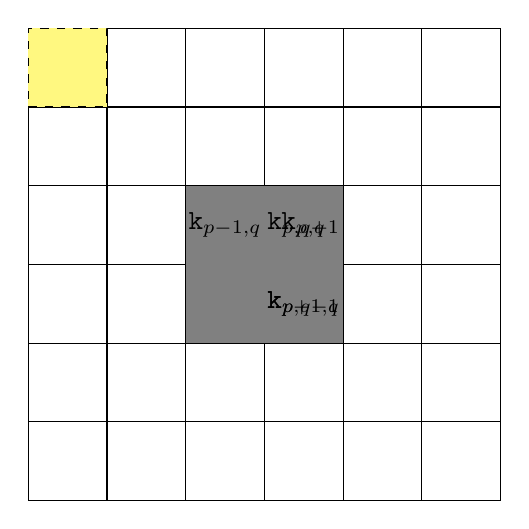
\begin{tikzpicture}
        % Define the coordinates for the fine elements
        \def\n{5} % Number of fine elements along one side
        
        % Draw the fine elements
        \foreach \i in {0,...,\n} {
            \foreach \j in {0,...,\n} {
                \node[draw, minimum size=1cm, fill=white] (f\i\j) at (\i,-\j) {};
            }
        }
        
        % Highlight the top-left corner fine element
        \node[draw, minimum size=1cm, fill=yellow!50, dashed] (hl) at (0,0) {};
        
        % Draw the oversampled coarse element
        \node[draw, minimum size=2cm, fill=gray, dashed] (coarse) at (0.5*\n,-0.5*\n) {};
        
        % Label the values of kappa
        \node at (0.5*\n+0.5, -0.5*\n+0.5) {$\mathtt{k}_{p,q}$};
        \node at (0.5*\n-0.5, -0.5*\n+0.5) {$\mathtt{k}_{p-1,q}$};
        \node at (0.5*\n+0.5, -0.5*\n-0.5) {$\mathtt{k}_{p+1,q}$};
        \node at (0.5*\n+0.5, -0.5*\n-0.5) {$\mathtt{k}_{p,q-1}$};
        \node at (0.5*\n+0.5, -0.5*\n+0.5) {$\mathtt{k}_{p,q+1}$};
    \end{tikzpicture}
    \caption{Illustration for the proof of Lemma \ref{lem:A_i}. The oversampled coarse element \( K_i^m \) with \( m = 2 \) is filled with gray and has a dashed border. The fine element in the top-left corner of \( K_i^m \) is highlighted.}
    \label{fig:illustration_lem_A_i}
\end{figure}

\end{document}